\setlength{\headheight}{13.59999pt}

This chapter is concerned with the method we have used to create semi-analytic models of planet wakes that encompass both the linear and non-linear disk response due to a perturbing planet as described in the previous chapter. 
Section \ref{sec:JOSS} introduces our Python package \textsc{wakeflow}, while sections \ref{sec:diskstruct}-\ref{sec:wakeprop} outline the theory and numerical methods it uses.

\section{Wakeflow: A Python Package For Semi-Analytic Models of Planet Wakes} \label{sec:JOSS}

This section has been published in the Journal of Open Source Science \fct and is publicly available here \fct

\subsubsection{Summary}

\textsc{wakeflow} is a Python package for generating semi-analytic models of the perturbations induced by planets embedded in gaseous circumstellar disks. 
These perturbationstake the form of a spiral shock wave \citep{ogilvie2002}, and are often called a "planet wake" in analogy with that produced by a boat in a lake.

\subsubsection{Statement of Need}

Detecting newly formed planets embedded in their disk is a challenging problem in the field of planet formation. 
A major area of progress in recent years isthe detection of planets by the gravitationally induced disturbance in theirhost disks. 
This disturbance, caused by the planet wake, manifests as a deviation in velocity from the bulk flow which may be measured through the Doppler shift of molecular lines \citep[eg.][]{perez2015, pinte2018a}. 
Such kinematic observations have been accurately reproduced through 3D fluid simulations of the planet-disk interaction, allowing for the inference of planet and disk properties \citep{pinte2018a, pinte2019}. 
However, these studies are computationally expensive.

\textsc{wakeflow} eases this computational cost by applying the theory of planet wake generation and propagation \citep{goldreich1979,goodman2001,rafikov2002a,bollati2021}to create semi-analytic models of planet wakes. 
\textsc{wakeflow} models are readily created in less than a minute on a modern laptop, as opposed to the hours of supercomputer time needed for 3D hydrodynamical simulations. 
The relatively low computational cost of \textsc{wakeflow}means that researchers can get an idea of whether planet-disk interactionscan explain their observations, and the disk and planet parameters needed, beforespending computer time on more detailed simulations.

\textsc{wakeflow} can interface with the radiative transfer code  \textsc{mcfost} \citep{pinte2006,pinte2009} in order to create synthetic observations of the semi-analytic models for direct comparison with observed continuum or line emission.

\textsc{wakeflow} is partially adapted from a previous Python code also written by us called \textsc{analytical\_kinks} [@Analytical\_Kinks]. 
\textsc{wakeflow} is intended to be a more complete, versatile and easy to use version of that code, and it obeys standard Python packaging conventions.
In addition, \textsc{wakeflow} can directly interface with \textsc{mcfost} while \textsc{analytical\_kinks} cannot.
At the time of writing, no other open source software packages exist to generate the perturbations induced by an embedded planet in a circumstellar disk using the semi-analytic theory of planet wakes.

Existing scientific publications focusing on detecting the kinematic signatures of planets that have used \textsc{wakeflow} or its predecessor \textsc{analytical\_kinks} include \citet{bollati2021}, \citet{calcino2022}, \citet{teague2022}, \citeauthor{garginreview} (in review) and \citeauthor{fasanoinprep.} (in prep.).

\subsubsection{Acknowledgements}

\textsc{wakeflow} relies on the following scientific Python packages: \textsc{numpy} \citep{harris2020}, \textsc{matplotlib} \citep{hunter2007}, \textsc{scipy} \citep{virtanen2020} and \textsc{astropy} \citep{astropycollaboration2022}.

\section{Disk Structure} \label{sec:diskstruct}

\section{Wake Formation} 

\subsection{The Shearing Sheet Approximation}

\section{Wake Propagation} 

\subsection{Power Law Disks}

\subsection{Velocity Perturbations} \label{sec:velocity_perts}

From \citet{rafikov2002a}, the conservation of the Riemann invariant $R_+$ gives for the radial velocity
\begin{align}
    u = 2\frac{c_0-c}{\gamma - 1}=-2\frac{c_0}{\gamma + 1} \psi, \label{eq:u_rafikov}
\end{align}
where we define $\psi$ as
\begin{align}
    \psi = \frac{\gamma+1}{\gamma-1} \frac{c - c_0}{c_0},
\end{align}
which is the sound speed perturbation with a constant scale factor. Following \citet{rafikov2002a}, we then derive an expression for $\psi$ in terms of the density perturbation $\chi$ by assuming that the gas obeys a locally polytropic equation of state given by 
\begin{align}
    P = P_0(r) \left[ \frac{\Sigma}{\Sigma_0(r)} \right]^\gamma. \label{eq:poly_EOS}
\end{align}
The sound speed is then
\begin{align}
    c^2 = \frac{\partial P}{\partial \Sigma} = c_0^2(r) \left[ \frac{\Sigma}{\Sigma_0(r)} \right]^{\gamma-1}.
\end{align}
\citet{rafikov2002a} then finds a relation between the density and sound speed perturbations, accurate to second order in $\psi$, found by expanding the above expression. 
This yields
\begin{align}
    \frac{\Sigma - \Sigma_0}{\Sigma_0} = \frac{2}{\gamma + 1}\psi + \frac{3 - \gamma}{\left( \gamma + 1  \right)^2} \psi^2 + \mathcal{O}(\psi^3). \label{eq:psi_exp}
\end{align}
Taking this expression to first order only, we write $u$ in terms of the density perturbation, and then in terms of $\chi$ by substituting Equation \feqr. 
\begin{align}
    u = - c_0 \frac{\Sigma - \Sigma_0}{\Sigma_0} = -2 \frac{c_0}{\gamma + 1} \frac{\chi}{g(r)}. \label{eq:ap_rad_vel}
\end{align}
Similarly, \citet{rafikov2002a} finds the azimuthal velocity as
\begin{align}
    v \approx -2 \frac{c_0^2}{\Delta\Omega r} \frac{1}{\gamma + 1} \psi, \label{eq:v_rafikov}
\end{align}
giving to first order in $\psi$
\begin{align}
    v \approx - \frac{c_0^2}{\Delta \Omega r} \frac{\Sigma - \Sigma_0}{\Sigma_0} = - \frac{2}{\gamma + 1} \frac{c_0^2}{\Delta \Omega r} \frac{\chi}{g(r)}. \label{eq:ap_az_vel}
\end{align}
Equations \ref{eq:ap_rad_vel} and \ref{eq:ap_az_vel} are the expressions used in \citet{bollati2021} to calculate the velocity perturbations in the non-linear regime. 
Since these are only accurate to first order in $\psi$, the assumption is made that $\psi \ll 1$; indeed \citet{bollati2021} notes that terms proportional to $\psi^2$ are discarded in the derivation of the Burgers evolution \feqr, and thus also in the calculation of $\chi$ from which $u$ and $v$ are calculated. 
However it is not clear that neglecting the most non-linear terms to calculate the density perturbation $\chi$ necissitates the truncation of the equation of state in the same way. 
Since we are in particular interested in the velocity perturbations, and in planet masses comparable to the thermal mass, we should check if the assumption that $\psi \ll 1$ holds.

We can derive an \textit{exact} expression for $\psi$ in terms of the density perturbation simply by rearranging Equation \ref{eq:poly_EOS}. We find
\begin{align}
    \psi = \frac{\gamma + 1}{\gamma - 1} \left[ \left( \frac{\Sigma-\Sigma_0}{\Sigma_0} +1  \right)^{(\psi-1)/2}  -1 \right],
\end{align}
which can be written equivalently in terms of $\chi$ using Equation \feqr giving
\begin{align}
    \psi = \frac{\gamma + 1}{\gamma - 1} \left[ \left( \frac{2}{\gamma + 1} \frac{\chi}{g(r)} +1  \right)^{(\psi-1)/2} -1 \right]. \label{eq:psi_exact}
\end{align}
We will use Equation \ref{eq:psi_exact} to check the aforementioned assumption that $\psi \ll 1$ in the non-linear regime solution. 
We construct three \textsc{wakeflow} models using dimensionless units, with embedded planet masses of $0.5, 1.0$ and $2.0 \, M_{\rm{th}}$ respectively, all placed in orbit around a $1 \, M_{\rm{\odot}}$ star at an orbital radius of $r=1$. 
For all models, we choose $p=2.25$ and $q=0.25$ such that $\Sigma \propto r^{-1}$, and an aspect ratio $H/r=0.1$ at $r=1$. 
Figure \ref{fig:psi_comparison} shows the values of $\psi$ for each of these models, and demonstrates that even for the lowest planet mass model the value of $\psi$ nearby the planet is as large as $\sim \hspace{-0.23em} 0.6$ and so the second order terms will clearly be important even in this case. 
For masses $\ge \hspace{-0.23em} M_\mathrm{th}$ the problem is even worse, as there are regions where $\psi \gtrsim 1$ causing the expansion given in Equation \ref{eq:psi_exp} to diverge.

\begin{figure}
    \centering
    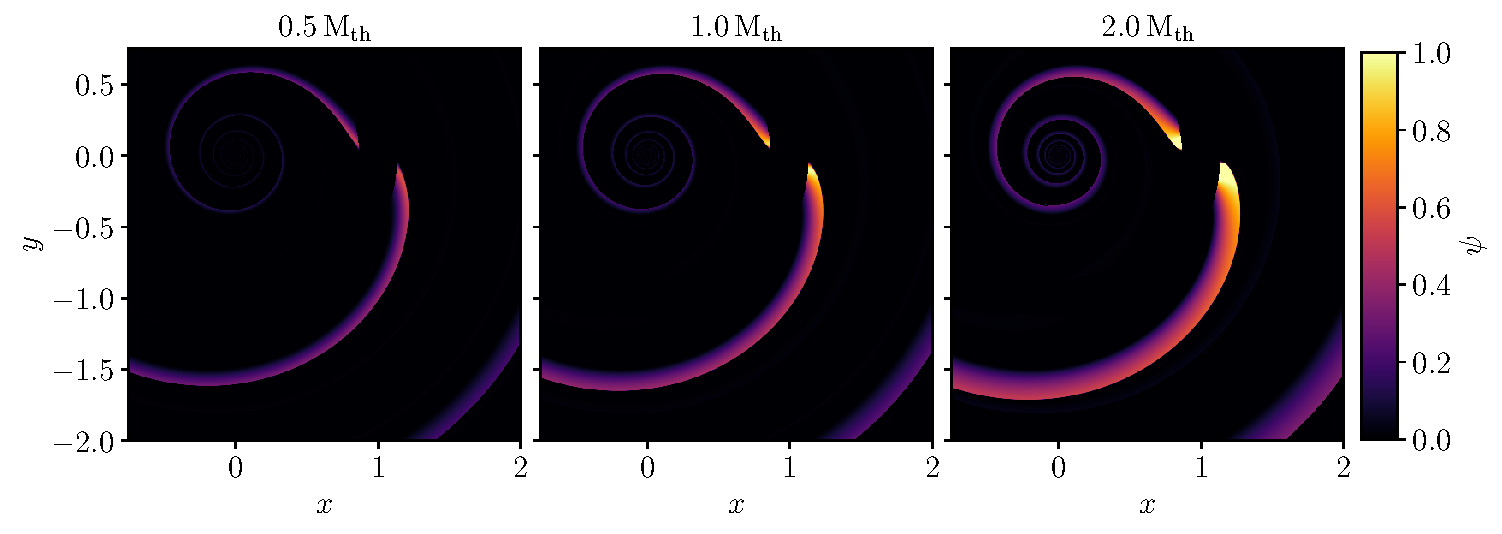
\includegraphics[width = 0.98\textwidth]{figures/psi 2.pdf}
    \caption{Comparison of the values of $\psi$ calculated from Equation \ref{eq:psi_exact} for three \textsc{wakeflow} models with planet masses of $0.5, 1.0$ and $2.0 \, M_{\rm{th}}$ respectively. Clearly one cannot assume that $\psi \ll 1$ even for the lowest mass model, especially nearby the planet. For the two larger masses, there are even regions where $\psi > 1$.}
    \label{fig:psi_comparison}
\end{figure}

To improve upon the velocity calculations used in \citet{bollati2021}, here we derive expressions for both $u$ and $v$ as functions of $\chi$ without truncating the equation of state to first order in $\psi$. This is as simple as substituting Equation \ref{eq:psi_exact} into Equations \ref{eq:u_rafikov} and \ref{eq:v_rafikov}, yielding
\begin{align}
    u(\chi) &= -2 \frac{c_0}{\gamma - 1} \left[ \left( \frac{2}{\gamma + 1} \frac{\chi}{g(r)} +1  \right)^{(\psi-1)/2} -1 \right] \\
    v(\chi) &\approx \frac{c_0}{\Delta\Omega r} u (\chi),
\end{align}
which are the expressions used to calculate the velocity perturbations in the non-linear regime in \textsc{wakeflow}. 

\begin{figure}
    \centering
    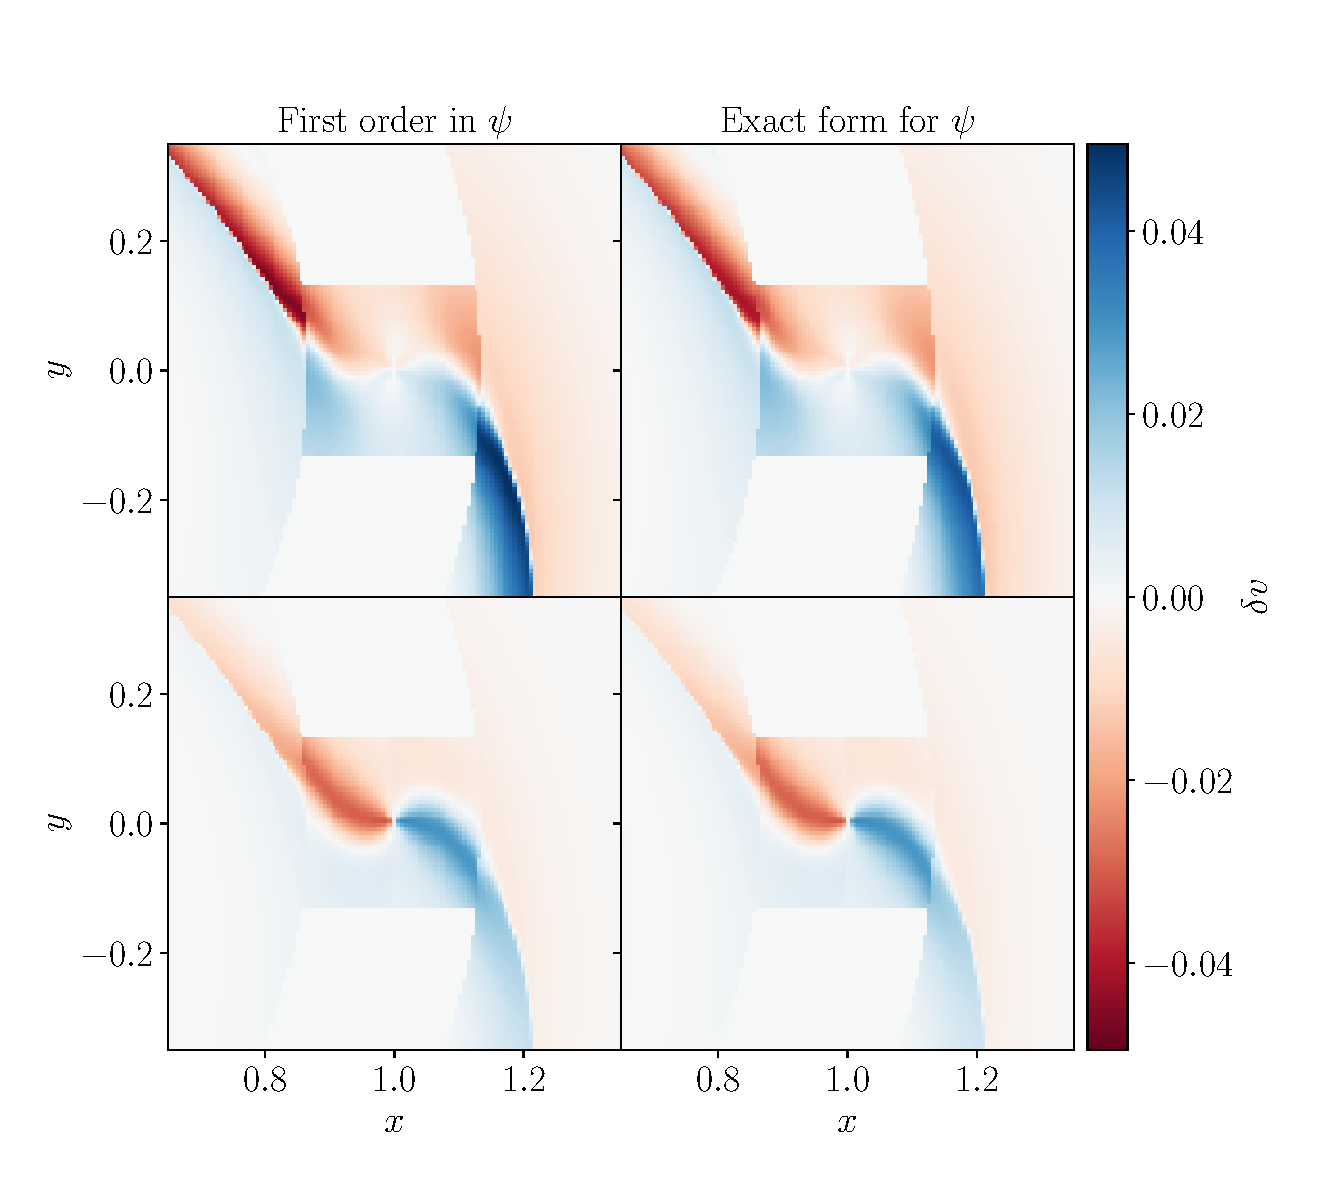
\includegraphics[width = 0.7\textwidth]{figures/0_5_mth.pdf}
    \caption{}
    \label{fig:0_5mth}
\end{figure}

\begin{figure}
    \centering
    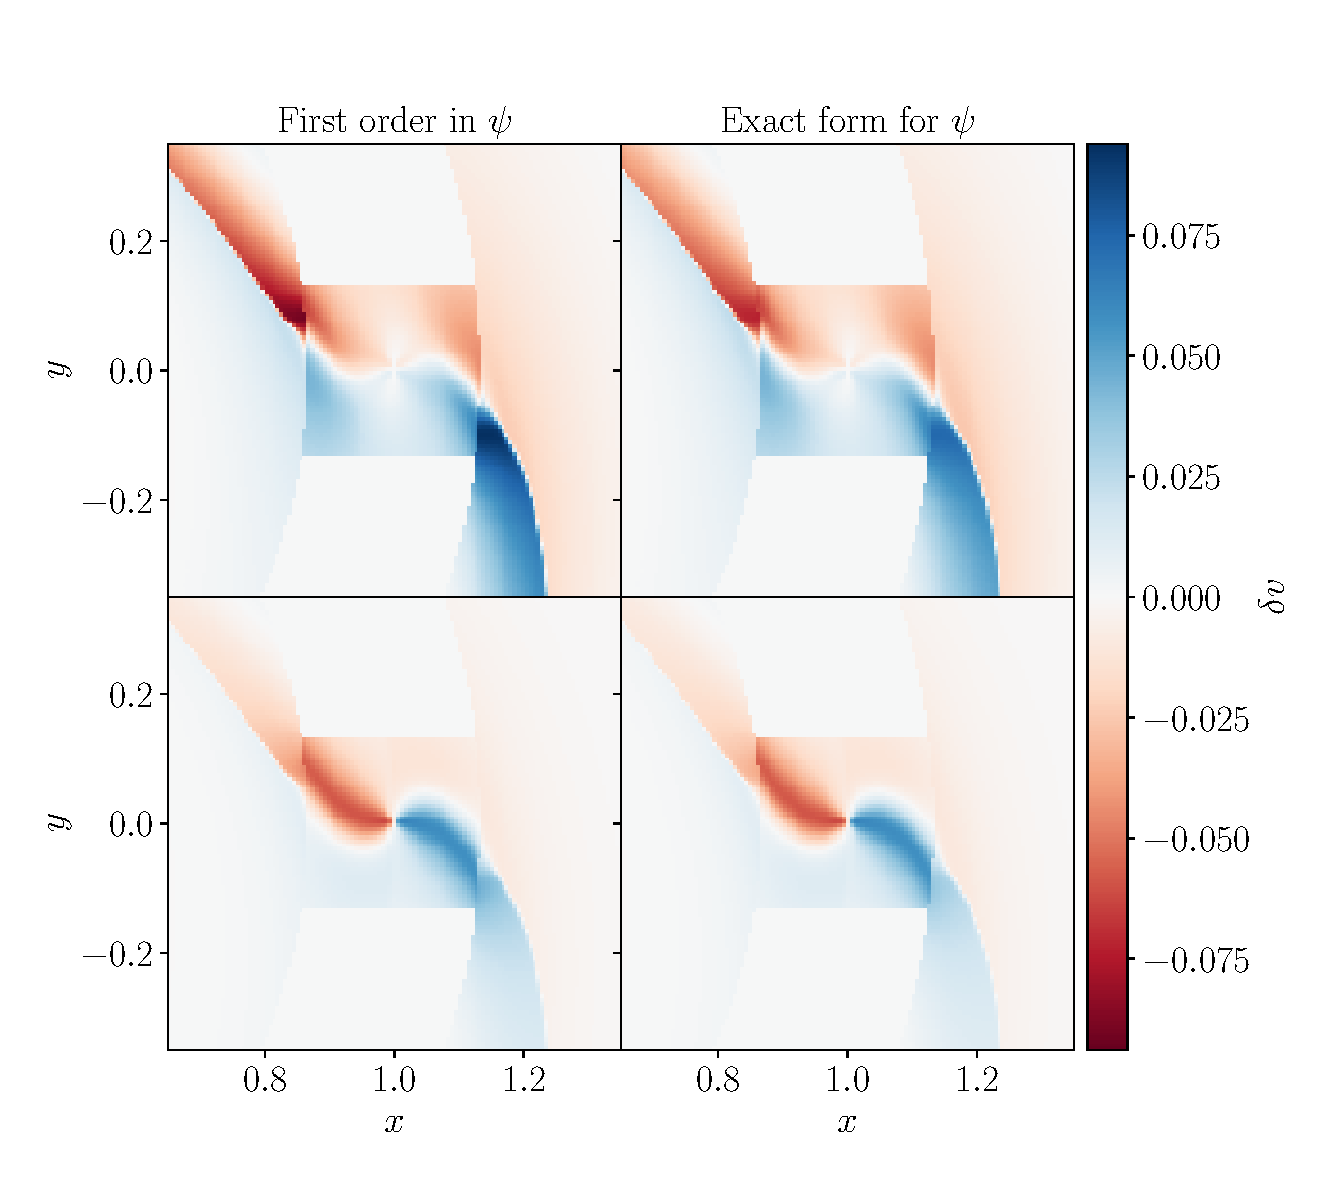
\includegraphics[width = 0.7\textwidth]{figures/1_0_mth.pdf}
    \caption{}
    \label{fig:1_0mth}
\end{figure}

\begin{figure}
    \centering
    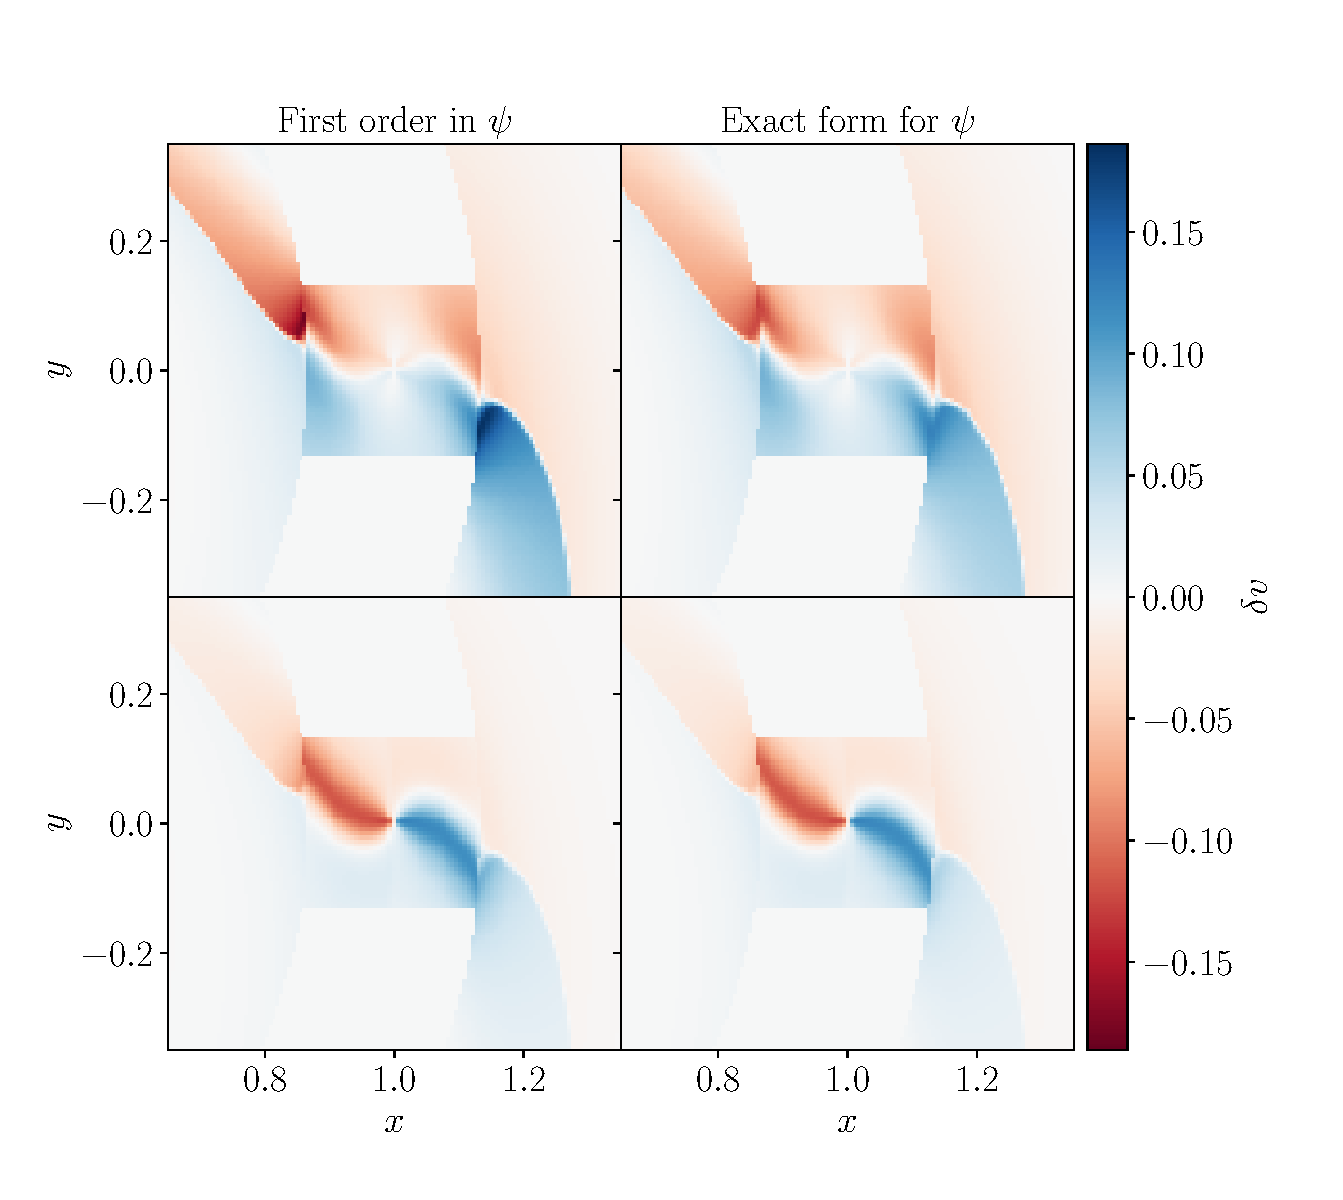
\includegraphics[width = 0.7\textwidth]{figures/2_0_mth.pdf}
    \caption{}
    \label{fig:2_0mth}
\end{figure}

\section{Synthetic Kinematic Observations}

\subsection{Predictions from 2D Models}

\subsection{3D Models}

\subsection{Radiation Transfer}